\section{Introduction}
Segmentation and clustering of large amounts of data is one of the main research fields of modern artificial intelligence.

The basis of our work is the collection of U.S. Census data in the year 1930 and fits into the process of digitalization of handwritten documents that characterizes our time. In this case we have scans of the census register and the main goal is to divide enrollees by State.

Document segmentation and extraction of the word corresponding to the State was developed previously by two of our colleagues in the course of \emph{Technology of Databases} and is the basis from which our work started.
The problem on which we have worked is the extraction of features from handwritten characters with the goal of creating clusters of similar words in order to facilitate the recognition by a human agent.

\begin{figure}[!ht]
\centering
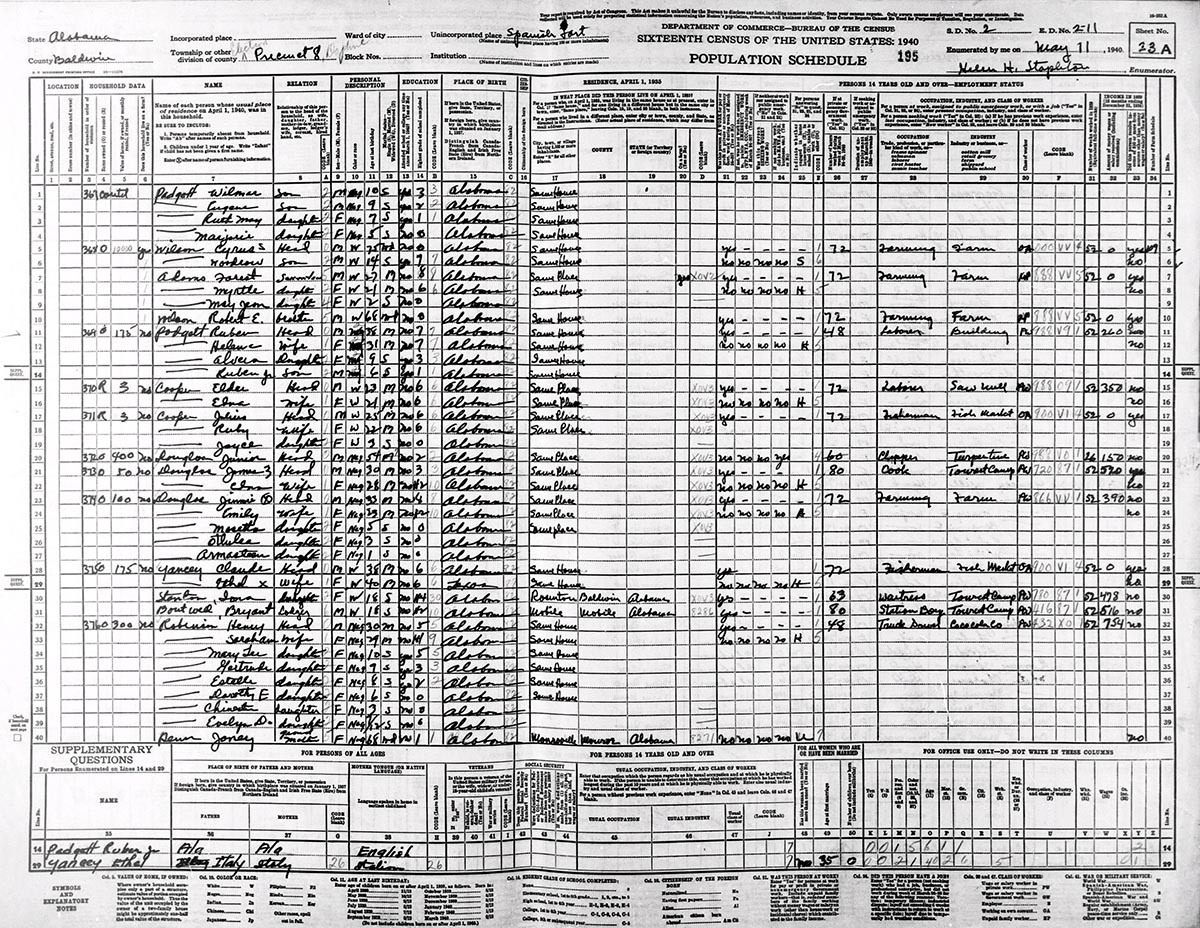
\includegraphics[width=0.6\textwidth]{images/img1.jpg}
\caption{An example of a table containing census data}
\end{figure}